% ------------------------- REVISADO
\mychapter{Resultados} 
\label{Cap:Resultados}

Neste capítulo, são apresentados os resultados da implementação e testes do \textit{software} RADARE, com foco na precisão dos dados reconciliados, no desempenho computacional em diferentes cenários de carga e na usabilidade da ferramenta, tanto no \textit{front-end} (menu e \textit{canvas}) quanto no \textit{back-end} (rotas, serviços e banco de dados).

Para facilitar a leitura e manter a fluidez do texto principal, todos os códigos desenvolvidos para o RADARE foram incluídos nos Anexos. Essa abordagem permite uma melhor organização do conteúdo, evitando que o texto principal seja interrompido por trechos extensos de código. Sempre que necessário, o texto principal indicará a referência ao anexo correspondente para consulta detalhada.

% ------------------------- REVISADO
\section{Resultados do desenvolvimento do \textit{front-end}}

O \textit{front-end} do projeto foi desenvolvido para oferecer uma interface intuitiva, facilitando a interação dos usuários com a ferramenta de modelagem. A interface permite a visualização dos fluxos de dados e modelos, além de possibilitar a execução da reconciliação. O \textit{front-end} é dividido em áreas principais: o menu, que gerencia as ações e funcionalidades; a \textit{sidebar} de informações de reconciliação; o gráfico dos dados reconciliados; e o \textit{canvas}, onde os nódulos conectados podem ser visualizados e manipulados diretamente pelos usuários.

% ------------------------- REVISADO
\subsection{Menu de controle da interface gráfica} 

A sessão de menu do RADARE apresenta ao usuário uma interface de fácil interação, permitindo a adição de componentes, o controle do fluxo de dados e o gerenciamento da visualização geral do sistema. Cada funcionalidade disponível no menu é descrita de maneira detalhada nas subseções a seguir, acompanhada por exemplos de código e imagens que ilustram sua implementação no contexto da ferramenta.

A biblioteca \textit{ReactFlow} \cite{reactflow} é fundamental para a manipulação dos nódulos no \textit{canvas} e foi significativamente adaptada para atender às necessidades específicas do projeto. As modificações realizadas garantem uma usabilidade eficiente, permitindo que os usuários adicionem e conectem os nódulos de forma dinâmica, com fluidez e precisão.

Cada nódulo inserido no \textit{canvas} possui uma estrutura personalizada, onde as conexões, denominadas \textit{handles}, são configuradas com características específicas, como estilo visual e lógica de interação. Essa personalização assegura que a visualização dos fluxos de dados seja clara e que sua manipulação seja intuitiva, facilitando o gerenciamento das operações dentro do sistema.

A Figura \ref{Fig:MenuImage} apresenta o \textit{menu} principal do sistema, destacando as opções para adição de nódulos ao \textit{canvas}. Através desse menu, o usuário pode inserir diferentes tipos de nódulos, como entradas, saídas e pontos de processamento de dados, além de opções como reconciliação de dados e ajustes de visualização. Cada funcionalidade foi projetada para que o usuário possa construir fluxos de dados industriais de maneira modular e interativa, proporcionando maior flexibilidade no gerenciamento e análise de grandes volumes de dados.

\begin{figure}[htbp]
    \centering
    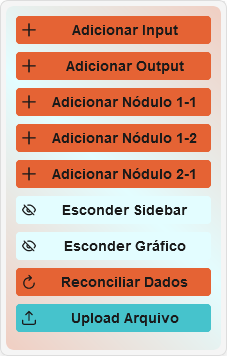
\includegraphics[width=0.4\textwidth]{figuras/menu-image.png}
    \caption{Menu principal do sistema RADARE (Fonte: próprio autor, 2024).}
    \label{Fig:MenuImage}
\end{figure}

% ------------------------- REVISADO
\subsubsection{Adicionar Input}

O botão \textbf{"Adicionar Input"} permite ao usuário inserir um novo nódulo de entrada no \textit{canvas}, representando um sensor ou uma fonte de dados no sistema industrial. Ao acionar esse botão, um nó de \textit{input} é adicionado ao \textit{canvas}, possibilitando a conexão desse ponto com outros nódulos do fluxo de dados. A implementação dessa funcionalidade utiliza a biblioteca ReactFlow \cite{reactflow}, o que elimina a necessidade de configurações customizadas iniciais e facilita a criação e manipulação dos nódulos no ambiente visual.

A Figura \ref{Fig:AddInputButton} ilustra o botão "Adicionar Input" na interface gráfica do sistema.

\begin{figure}[htbp]
    \centering
    
\includegraphics[width=0.4\textwidth]{figuras/add-input-button.png}
    \caption{Botão de adicionar \textit{input} no menu (Fonte: próprio autor, 2024).}
    \label{Fig:AddInputButton}
\end{figure}

% ------------------------- REVISADO
\subsubsection{Adicionar output}

O botão \textbf{"Adicionar Output"} permite ao usuário inserir um novo nódulo de saída no \textit{canvas}. Esse \textit{output} representa um destino ou ponto final para os dados no sistema industrial, como a exportação de resultados processados ou a visualização de dados reconciliados. Ao acionar o botão, um novo nó de \textit{output} é adicionado ao \textit{canvas}, possibilitando sua conexão com outros nódulos de processamento ou entrada no fluxo de dados. Assim como ocorre com o \textit{input}, a implementação dessa funcionalidade também utiliza a biblioteca ReactFlow \cite{reactflow}, eliminando a necessidade de customização de comportamentos iniciais.

A Figura \ref{Fig:AddOutputButton} mostra o botão "Adicionar Output" na interface, permitindo ao usuário inserir nódulos de saída no fluxo de dados.

\begin{figure}[htbp]
    \centering
    
\includegraphics[width=0.4\textwidth]{figuras/add-output-button.png}
    \caption{Botão de adicionar output no menu (Fonte: próprio autor, 2024).}
    \label{Fig:AddOutputButton}
\end{figure}

% ------------------------- REVISADO
\subsubsection{Adicionar nódulo 1-1}

O botão \textbf{"Adicionar Nódulo 1-1"} permite ao usuário inserir um novo nódulo de transição no \textit{canvas}. Esse nódulo atua como um ponto intermediário no fluxo de dados, podendo representar sensores, transformações ou outros elementos de processo. Ao clicar no botão, o nódulo é adicionado ao \textit{canvas}, permitindo ao usuário conectá-lo com outros nódulos.

A lógica para adicionar este nódulo foi desenvolvida de forma personalizada, especificando o tipo de conexão, a quantidade de pontos de conexão (\textit{handles}), além do estilo visual e da posição no \textit{canvas}, garantindo que o comportamento do nódulo se ajuste adequadamente ao fluxo de dados esperado. O trecho principal do código responsável pela criação desse nódulo pode ser encontrado em sua totalidade no \textbf{Anexo \ref{Anexo:frontCodeNodeOneOne}}.

\begin{figure}[htbp]
    \centering
    
\includegraphics[width=0.4\textwidth]{figuras/add-node11-button.png}
    \caption{Botão de adicionar Nódulo 1-1 no menu (Fonte: próprio autor, 2024).}
    \label{Fig:AddNodeOneOneButton}
\end{figure}

% ------------------------- REVISADO
\subsubsection{Adicionar nódulo 1-2}

O botão \textbf{"Adicionar Nódulo 1-2"} permite ao usuário inserir um nódulo de transição que recebe uma única entrada e gera duas saídas no \textit{canvas}. Este tipo de nódulo é particularmente útil em cenários onde um único ponto de dados precisa ser bifurcado para diferentes processos ou análises. Ao ser adicionado, o nódulo facilita o roteamento de dados para dois fluxos distintos, mantendo a integridade e a flexibilidade do processo.

A lógica para este nódulo foi customizada para suportar uma conexão de entrada e duas saídas, com o código responsável definindo os \textit{handles} (pontos de conexão), a posição e o estilo visual no \textit{canvas}. Assim como no caso do nódulo 1-1, o comportamento é ajustado para garantir uma integração fluida no fluxo de dados. O trecho principal do código responsável pela criação desse nódulo pode ser encontrado em sua totalidade no \textbf{Anexo \ref{Anexo:frontCodeNodeOneTwo}}.

A Figura \ref{Fig:AddNodeOneTwoButton} ilustra o botão "Adicionar Nódulo 1-2" disponível no menu do sistema.

\begin{figure}[htbp]
    \centering
    
\includegraphics[width=0.4\textwidth]{figuras/add-node12-button.png}
    \caption{Botão de adicionar Nódulo 1-2 no menu (Fonte: próprio autor, 2024).}
    \label{Fig:AddNodeOneTwoButton}
\end{figure}

% ------------------------- REVISADO
\subsubsection{Adicionar nódulo 2-1}

O botão \textbf{"Adicionar Nódulo 2-1"} permite ao usuário inserir um nódulo de transição que recebe duas entradas e gera uma única saída no \textit{canvas}. Esse nódulo é ideal para processos em que múltiplas fontes de dados precisam ser combinadas ou integradas, antes de continuar o fluxo. Ao ser adicionado, o nódulo permite a fusão de duas linhas de dados, garantindo que as informações de entrada sejam processadas de forma conjunta, antes de seguirem para a próxima etapa.

A lógica para este nódulo foi desenvolvida de maneira personalizada, permitindo a adição de dois pontos de conexão de entrada e um ponto de saída. O código responsável configura os \textit{handles}, define o estilo visual e posiciona o nódulo no \textit{canvas}, assegurando que ele atenda às necessidades de integração e processamento combinados dentro do fluxo de dados. O trecho principal do código responsável pela criação desse nódulo pode ser encontrado em sua totalidade no \textbf{Anexo \ref{Cap:NodeTwoOneCode}}.

A Figura \ref{Fig:AddNodeTwoOneButton} mostra o botão "Adicionar Nódulo 2-1" presente no menu da interface do sistema.

\begin{figure}[htbp]
    \centering
    
\includegraphics[width=0.4\textwidth]{figuras/add-node21-button.png}
    \caption{Botão de adicionar Nódulo 2-1 no menu (Fonte: próprio autor, 2024).}
    \label{Fig:AddNodeTwoOneButton}
\end{figure}

% ------------------------- REVISADO
\subsubsection{Reconciliar dados}

O botão \textbf{"Reconciliar Dados"} executa o processo de reconciliação dos dados conectados no \textit{canvas}. Ao ser acionado, o sistema analisa os nódulos interconectados e realiza a reconciliação dos dados utilizando o método dos multiplicadores de Lagrange. Esse processo ajusta as discrepâncias entre os valores medidos e os valores reconciliados, garantindo que as restrições impostas pelos balanços de massa e energia sejam respeitadas.

A lógica por trás desse botão foi desenvolvida para percorrer os nódulos conectados no \textit{canvas}, extrair os dados necessários e enviá-los ao \textit{back-end}. No \textit{back-end}, o algoritmo de reconciliação é executado, processando os dados conforme as regras definidas, e os resultados são retornados ao \textit{front-end}, onde os dados reconciliados são exibidos no fluxo visual do \textit{canvas}. O trecho principal do código responsável por essa funcionalidade pode ser encontrado em sua totalidade no \textbf{Anexo \ref{Cap:ReconcileDataCode}}.

A Figura \ref{Fig:ReconcileButton} ilustra o botão "Reconciliar Dados" na interface do sistema.

\begin{figure}[htbp]
    \centering
    
\includegraphics[width=0.4\textwidth]{figuras/reconcile-data-button.png}
    \caption{Botão de reconciliar dados no menu (Fonte: próprio autor, 2024).}
    \label{Fig:ReconcileButton}
\end{figure}

% ------------------------- REVISADO
\subsubsection{Esconder gráfico das reconciliações}

O botão \textbf{"Esconder Gráfico das Reconciliações"} permite ao usuário ocultar o gráfico que exibe os resultados das reconciliações de dados, proporcionando uma interface mais organizada e com maior espaço para outros elementos do processo. Ao ativar essa função, o gráfico é temporariamente removido do \textit{dashboard}, mas os dados reconciliados permanecem disponíveis no sistema, permitindo que o usuário possa reexibi-los quando necessário. A lógica implementada para esse botão utiliza um simples operador ternário para alternar a visibilidade do gráfico, sem interferir nos demais componentes ou no fluxo dos dados processados. Dada a simplicidade da implementação, não é necessário incluir um anexo de código.

A Figura \ref{Fig:Recon} ilustra o botão "Esconder Gráfico das Reconciliações" na interface gráfica.

\begin{figure}[htbp] \centering 
\includegraphics[width=0.4\textwidth]{figuras/hide-graphbar-button.png} \caption{Botão de esconder gráfico das reconciliações (Fonte: próprio autor, 2024).} \label{Fig:Recon} \end{figure}

% ------------------------- REVISADO
\subsubsection{Esconder \textit{Sidebar} de Informações}

O botão \textbf{"Esconder Sidebar de Informações"} permite ao usuário ocultar a barra lateral que exibe informações detalhadas sobre os nódulos e fluxos no \textit{canvas}, liberando mais espaço para visualização e manipulação em fluxos complexos. A lógica dessa funcionalidade é simples, utilizando ternários em SCSS para alternar estilos e \textit{useState} do React para controlar a visibilidade da \textit{sidebar} sem perda de dados. O usuário pode reexibi-la a qualquer momento com as informações preservadas, garantindo uma interface adaptável. Não há necessidade de anexo com código, pois a implementação é direta.

A Figura \ref{Fig:HideSidebarButton} ilustra o botão "Esconder Sidebar de Informações" \ na interface gráfica do sistema.

\begin{figure}[htbp]
    \centering
    
\includegraphics[width=0.4\textwidth]{figuras/hide-sidebar-button.png}
    \caption{Botão de esconder a sidebar de informações (Fonte: próprio autor, 2024).}
    \label{Fig:HideSidebarButton}
\end{figure}

% ------------------------- REVISADO
\subsubsection{Upload de Arquivos em CSV}

O botão \textbf{"Upload de Arquivos CSV"} permite ao usuário importar dados de medições diretamente para o sistema, integrando informações externas ao fluxo de trabalho. Arquivos CSV contendo dados de sensores e variáveis do processo industrial podem ser carregados no RADARE, onde são processados e utilizados nas etapas de reconciliação para análise e correção.

A funcionalidade valida o formato e conteúdo dos arquivos, garantindo que os dados estejam estruturados para integração ao banco de dados e processamento. O código dessa funcionalidade pode ser encontrado no \textbf{Anexo \ref{Anexo:UploadCSVLogic}}, onde é detalhada a implementação do upload e validação dos arquivos CSV.

A Figura \ref{Fig:UploadCSVButton} mostra o botão "Upload de Arquivos CSV" na interface do sistema.

\begin{figure}[htbp]
    \centering
    
\includegraphics[width=0.4\textwidth]{figuras/upload-csv-button.png}
    \caption{Botão de upload de arquivos CSV (Fonte: próprio autor, 2024).}
    \label{Fig:UploadCSVButton}
\end{figure}

% ------------------------- REVISADO
\subsection{\textit{Canvas} do sistema}

O \textit{canvas} é a área principal da interface do RADARE, onde o usuário pode visualizar, conectar e manipular os nódulos para configurar o fluxo de dados industrial. É nesse espaço que o usuário constrói e ajusta os fluxos de trabalho, interligando entradas, saídas e pontos de processamento. A interação no \textit{canvas} é dinâmica e permite a personalização dos fluxos conforme as necessidades do processo.

A Figura \ref{Fig:EmptyCanvas} mostra um exemplo do \textit{canvas} com vários nódulos conectados, oferecendo uma visão geral de como os elementos podem ser arranjados e manipulados visualmente.

\begin{figure}[htbp]
    \centering
    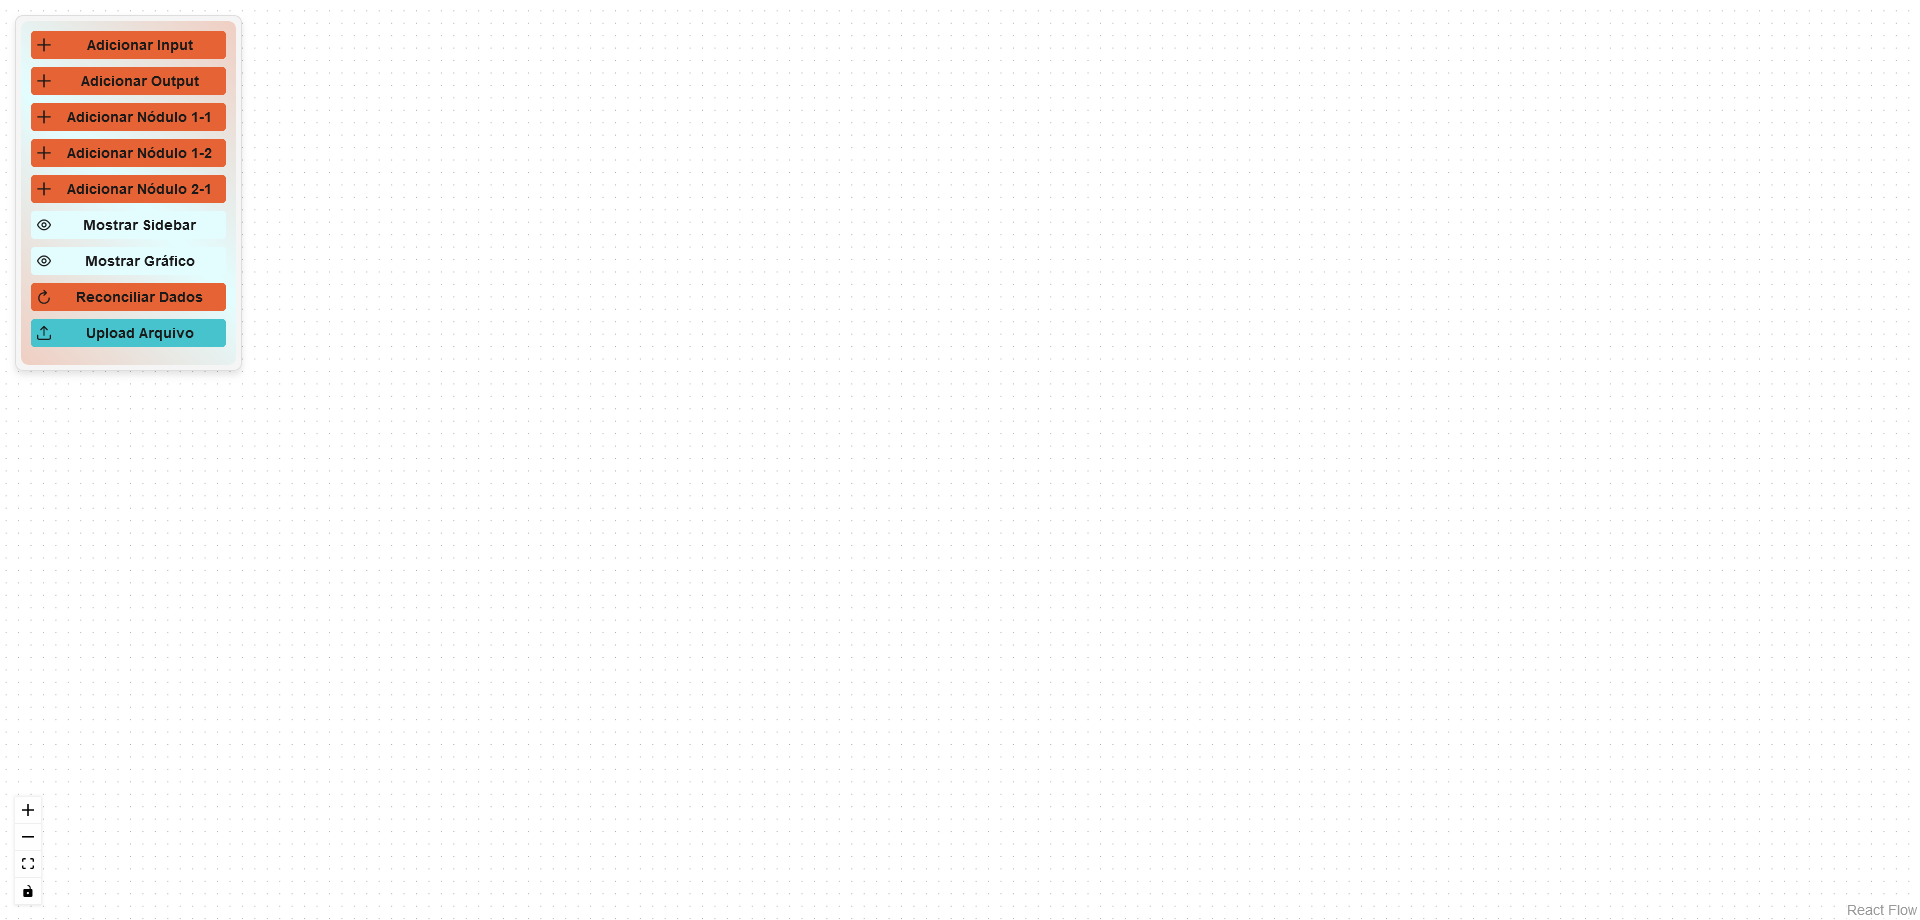
\includegraphics[width=0.8\textwidth]{figuras/empty-canvas.png}
    \caption{Exemplo da área de trabalho no canvas do RADARE (Fonte: próprio autor, 2024).}
    \label{Fig:EmptyCanvas}
\end{figure}

% ------------------------- REVISADO
\subsubsection{Lógica de conexão entre os nódulos no \textit{canvas}}

O sistema permite que o usuário estabeleça conexões visuais entre os nódulos, representando o fluxo de dados entre diferentes pontos de um processo industrial. Essas conexões são fundamentais para assegurar que os dados fluam corretamente entre os elementos do \textit{canvas}, como entradas, saídas e pontos de processamento.

A Figura \ref{Fig:NodeConnections} ilustra a conexão de dois nódulos no \textit{canvas}, demonstrando como o usuário pode arrastar e soltar as conexões de forma intuitiva. O usuário também pode ajustar e mover essas conexões entre os nódulos. Cada conexão entre os nódulos possui um valor e uma tolerância associados, que podem ser modificados diretamente com um duplo clique na linha de conexão, permitindo ao usuário ajustar os parâmetros conforme necessário. Além disso, as conexões recebem nomes gerados automaticamente para facilitar a distinção entre as diferentes \textit{tags}. O trecho principal do código responsável pela criação dessa funcionalidade está disponível no \textbf{Anexo \ref{Anexo:frontCodeNodeTwoOne}}.

\begin{figure}[htbp]
    \centering
    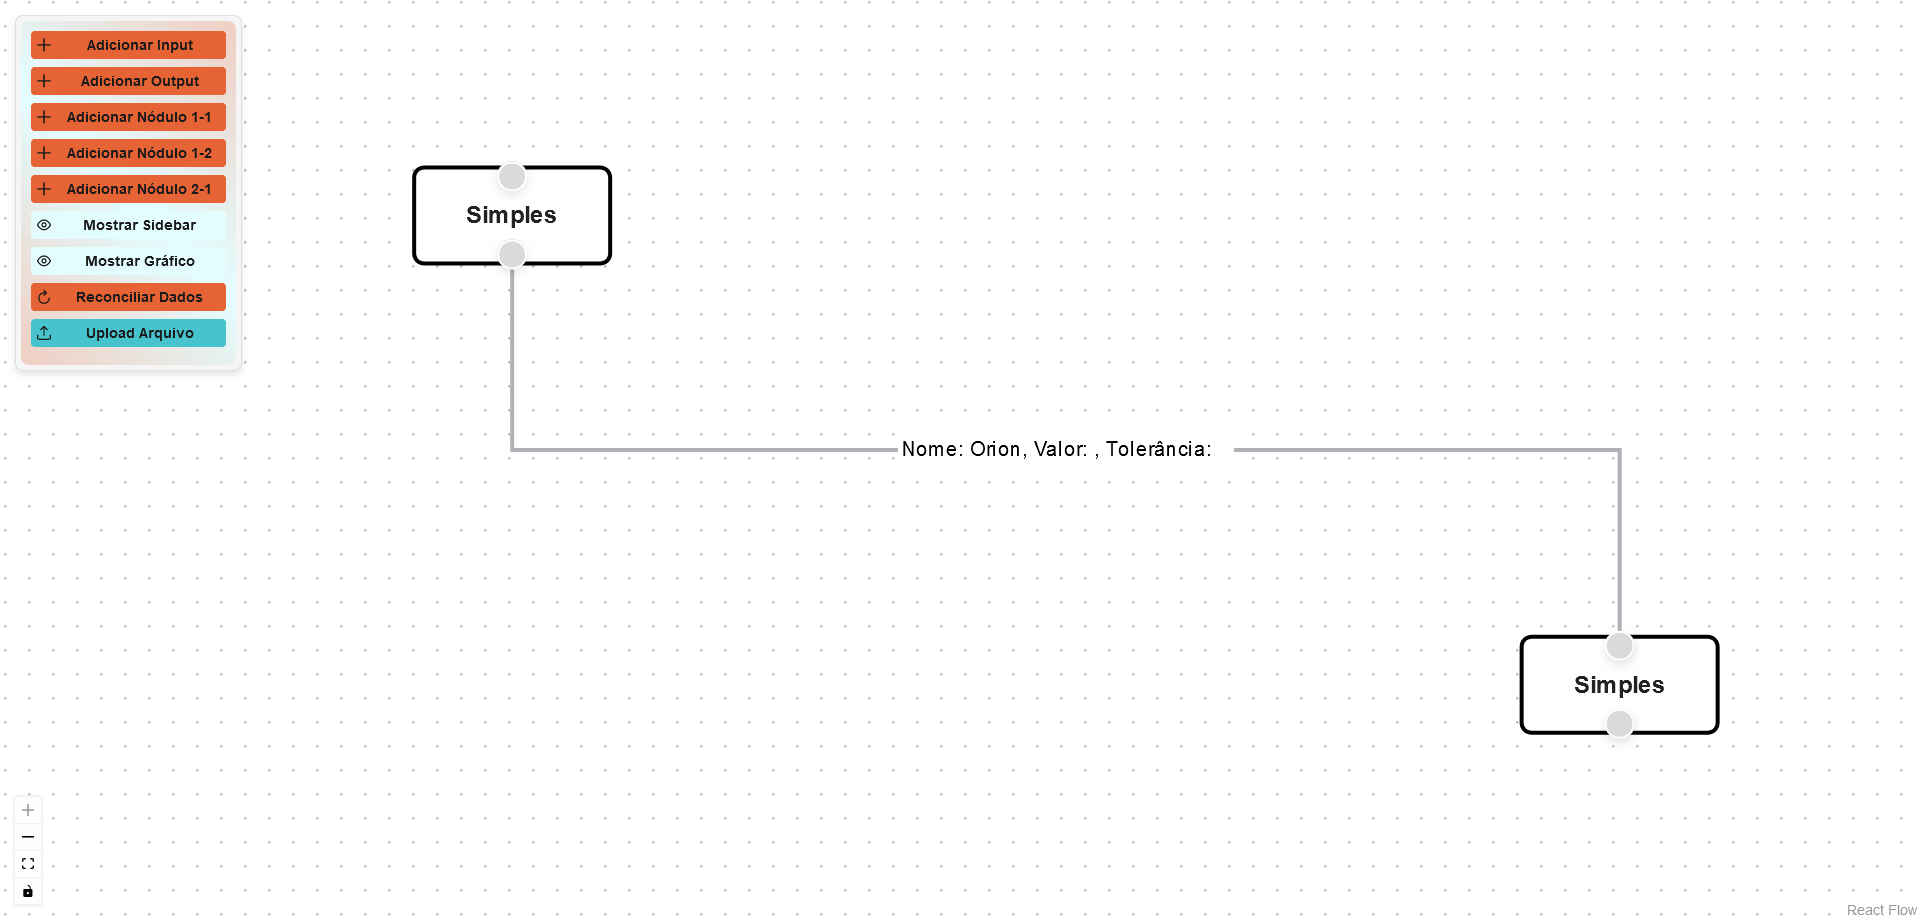
\includegraphics[width=0.8\textwidth]{figuras/node-connection-example.png}
    \caption{Exemplo de conexão entre nódulos no \textit{canvas} (Fonte: próprio autor, 2024).}
    \label{Fig:NodeConnections}
\end{figure}

% ------------------------- REVISADO
\subsection{Interface do gráfico de reconciliação de dados}

A interface de gráfico de reconciliação de dados no RADARE permite ao usuário comparar diretamente os valores medidos e reconciliados, facilitando a identificação de discrepâncias. O gráfico exibe as variações dos dados em função das interações realizadas, ajudando a avaliar o progresso e situação dos dados reconciliados.

A Figura \ref{Fig:ReconciliationGraph} mostra um exemplo de gráfico de interações versus valores na interface do RADARE. O código responsável pela exibição desse gráfico está no \textbf{Anexo \ref{Anexo:ReconciliationGraph}}.

\begin{figure}[htbp]
    \centering
    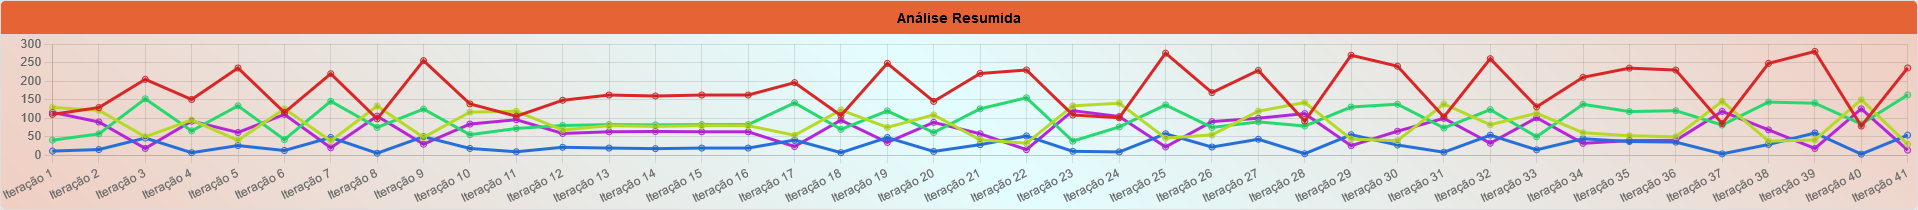
\includegraphics[width=1\textwidth]{figuras/interface-grafico.png}
    \caption{Exemplo do gráfico de reconciliações por interação (Fonte: próprio autor, 2024).}
    \label{Fig:ReconciliationGraph}
\end{figure}

% ------------------------- REVISADO
\subsection{Interface da \textit{sidebar} de informações do sistema}

A \textit{sidebar} de informações do sistema no RADARE serve como um painel auxiliar para exibir informações detalhadas sobre os nódulos e fluxos configurados no \textit{canvas}. Ela permite ao usuário acessar dados adicionais e propriedades de cada elemento, facilitando o monitoramento e o ajuste preciso dos componentes do fluxo de trabalho industrial. A \textit{sidebar} também possibilita uma navegação rápida entre os nódulos e fornece opções para personalização, promovendo uma experiência de uso intuitiva e eficiente.

A Figura \ref{Fig:SidebarInterface} mostra um exemplo da \textit{sidebar} com detalhes de nódulos selecionados, como as informações organizadas para facilitar a edição e o monitoramento dos elementos visuais do \textit{canvas}. O código que rege a lógica por trás deste componente está disponível no \textbf{Anexo \ref{Anexo:CodigoSidebar}}.

\begin{figure}[htbp]
    \centering
    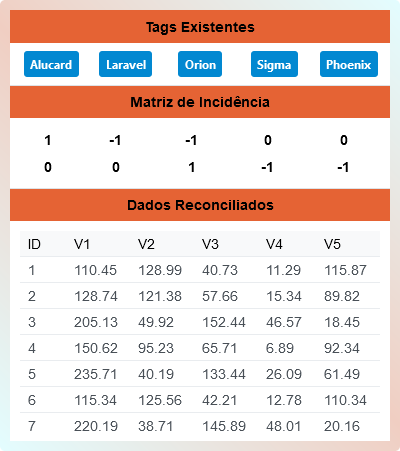
\includegraphics[width=0.4\textwidth]{figuras/interface-sidebar.png}
    \caption{Exemplo da \textit{sidebar} de informações do sistema no RADARE, exibindo dados e opções de configuração de nódulos (Fonte: próprio autor, 2024).}
    \label{Fig:SidebarInterface}
\end{figure}

% ------------------------- REVISADO
\subsection{Resultados finais do front-end em sua visualização completa}

O desenvolvimento do \textit{front-end} do RADARE culminou em uma tela inicial funcional e intuitiva, integrando todas as funcionalidades discutidas anteriormente. A área do \textit{canvas} serve como o núcleo da interface, permitindo que o usuário visualize, conecte e manipule os nódulos para configurar o fluxo de dados industrial de maneira personalizada. É nesse espaço que os fluxos de trabalho são estruturados, com entradas, saídas e pontos de processamento conectados em harmonia para atender às necessidades específicas dos processos industriais.

A Figura \ref{Fig:CanvasArea} apresenta o \textit{canvas} com vários nódulos interligados, proporcionando uma visão satisfatória de como os elementos podem ser organizados e ajustados para criar um fluxo de trabalho viável e eficiente. Cada nódulo desempenha uma função distinta dentro do sistema, e as conexões entre eles representam o fluxo de dados que o RADARE processa e reconcilia. 

\begin{figure}[htbp]
    \centering
    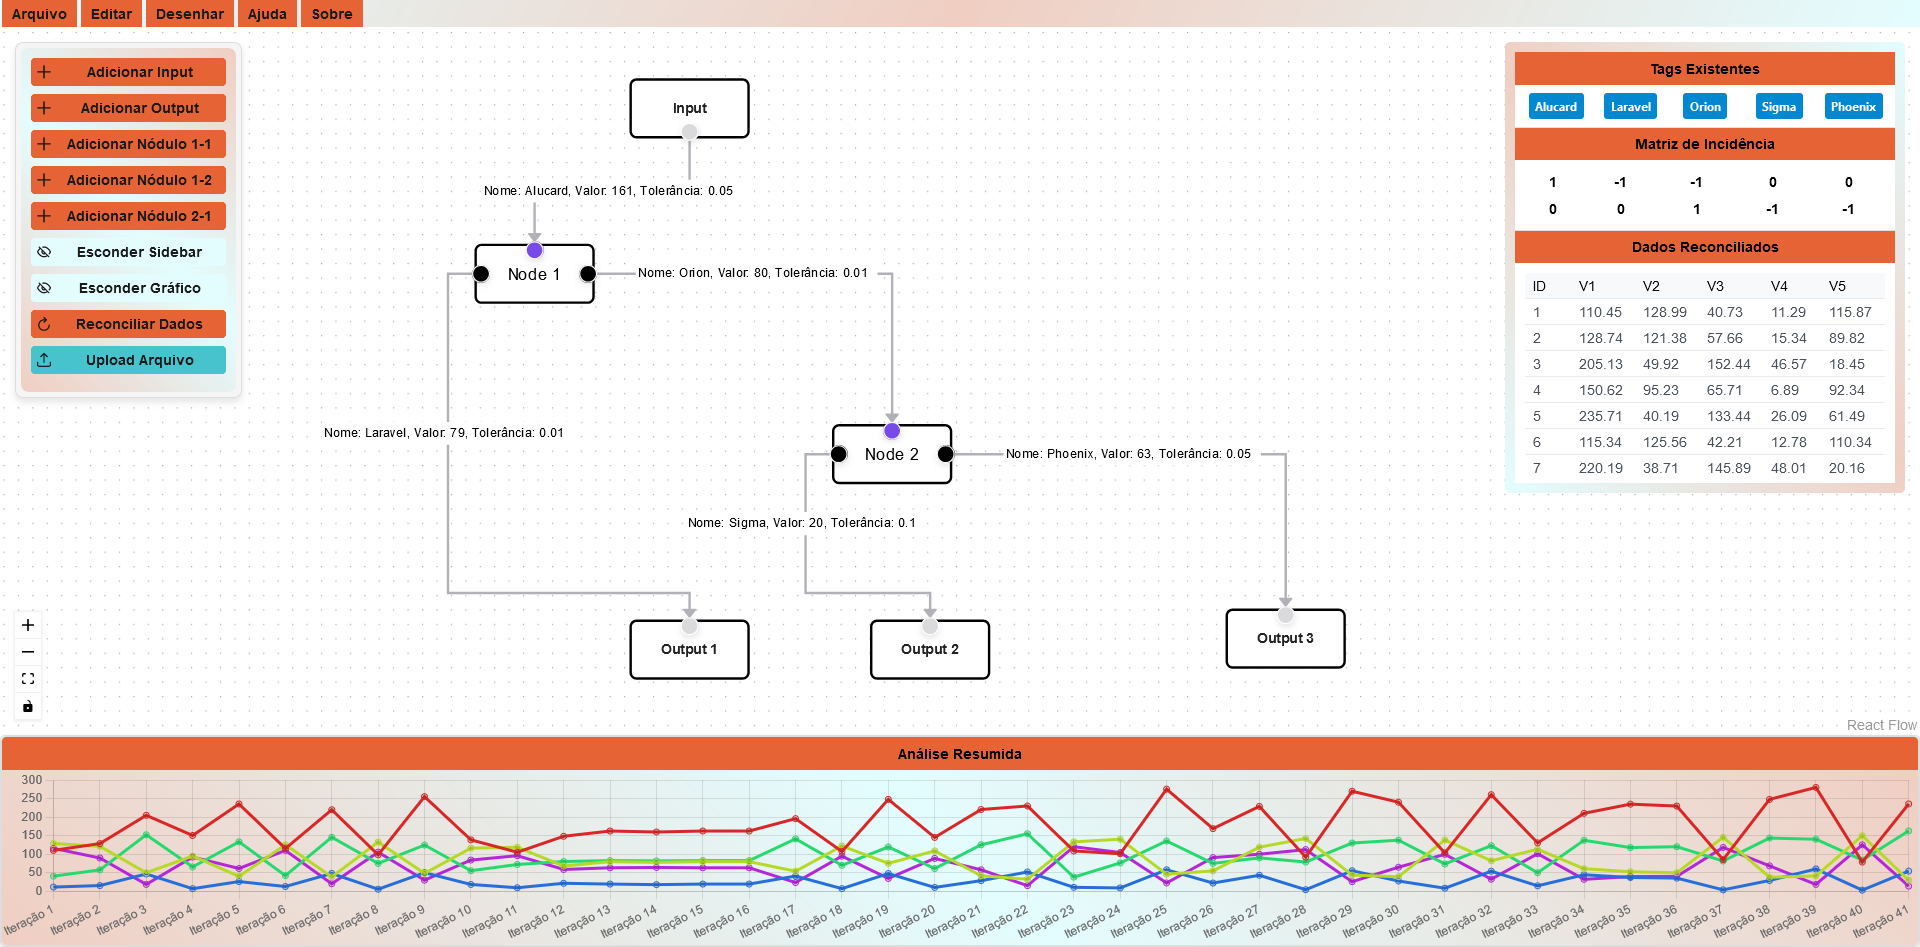
\includegraphics[width=0.8\textwidth]{figuras/interface-completa.png}
    \caption{Exemplo da área de trabalho no canvas do RADARE (Fonte: próprio autor, 2024).}
    \label{Fig:CanvasArea}
\end{figure}

% ------------------------- REVISADO
\section{Resultados do desenvolvimento do \textit{back-end}}

O \textit{back-end} do RADARE foi desenvolvido em \textit{Python} com o \textit{framework} Flask. Essa camada gerencia as requisições da interface, processa os dados submetidos, realiza os cálculos de reconciliação com o método dos multiplicadores de Lagrange, armazena os dados processados de forma segura e comunica-se com o \textit{front-end} para exibir os resultados. A estrutura foi configurada para responder de forma eficiente às operações, garantindo comunicação ágil entre as partes do sistema.

% ------------------------- REVISADO
\subsection{Desenvolvimento das interfaces RESTful de comunicação entre os sistemas}

As interfaces RESTful foram projetadas para garantir uma comunicação eficiente e segura entre o \textit{front-end} e o \textit{back-end} do sistema RADARE. Cada rota foi estruturada para facilitar o envio e recebimento de dados e a execução dos processos de reconciliação. A seguir, são descritas as rotas implementadas, com exemplos de código e explicações sobre cada \textit{endpoint} e sua importância na integração dos componentes do sistema.

% ------------------------- REVISADO
\subsubsection{Interface RESTful para Obter Dados Reconciliados: \texttt{GET /reconciled-data}}

A rota \texttt{GET /reconciled-data} permite ao usuário recuperar os dados reconciliados armazenados no banco de dados. Quando acionada, esta rota consulta o banco e retorna os valores ajustados, que são exibidos na interface gráfica para visualização e análise.

Esse processo envolve uma consulta ao banco de dados, onde os resultados das reconciliações são armazenados após o processamento. Os dados reconciliados refletem os valores ajustados com base no método dos multiplicadores de Lagrange, aplicados durante a fase de reconciliação. O código completo para a implementação desta rota pode ser consultado no \textbf{Anexo \ref{Anexo:CodigoFunctionGetReconciledData}}.

% ------------------------- REVISADO
\subsubsection{Interface RESTful para Obter Dados Reconciliados: \texttt{GET /reconciled-data}}

A rota \texttt{GET /reconciled-data} permite ao usuário recuperar os dados reconciliados armazenados no banco de dados. Quando acionada, esta rota consulta o banco e retorna os valores ajustados, que são exibidos na interface gráfica para visualização e análise.

Esse processo envolve uma consulta ao banco de dados, onde os resultados das reconciliações são armazenados após o processamento. Os dados reconciliados refletem os valores ajustados com base no método dos multiplicadores de Lagrange, aplicados durante a fase de reconciliação.

% ------------------------- REVISADO
\subsubsection{Endpoint RESTful para Verificação de Conexão: \texttt{GET /health}}

A rota \texttt{GET /health} é um \textit{endpoint} simples de verificação da qualidade da conexão no sistema RADARE. Ela permite que o \textit{front-end} e o \textit{back-end} verifiquem rapidamente se a comunicação está ativa e funcional. Ao acessar esta rota, o sistema responde com uma confirmação imediata, indicando que a conexão está estável e o \textit{back-end} está operacional. Esse \textit{endpoint} é útil para monitoramento básico e para identificar eventuais falhas de conexão antes de iniciar operações mais complexas.

% ------------------------- REVISADO
\subsection{Serviço de Reconciliação de Dados}

O serviço de reconciliação de dados no \textit{back-end} do RADARE é responsável por implementar a lógica de negócio e executar os cálculos de reconciliação, garantindo que os dados sejam processados corretamente antes de serem armazenados no banco de dados ou enviados à interface. Esse serviço utiliza o método dos multiplicadores de Lagrange para assegurar que as restrições de balanço de massa e energia sejam respeitadas, assegurando a consistência dos dados processados.

O código principal desse serviço, detalhado no \textbf{Anexo \ref{Anexo:CodigoReconciliacaoDados}}, exemplifica a implementação do método de reconciliação e a integração com o banco de dados para o armazenamento dos resultados.

% ------------------------- REVISADO
\section{Resultados do Desenvolvimento do Banco de Dados}

O banco de dados do sistema RADARE, implementado em PostgreSQL, armazena todas as informações essenciais para a execução dos processos de reconciliação de dados industriais, gerenciamento de usuários e rastreamento de atividades. A modelagem foi simplificada para garantir integridade e eficiência na consulta e manipulação dos dados, atendendo às necessidades específicas do sistema sem complexidade excessiva.

A tabela de dados de processos industriais (\autoref{tab:processDataTable}) armazena informações fundamentais para o funcionamento do RADARE, incluindo medições de sensores e resultados das reconciliações. Essa estrutura organiza os dados de forma clara, garantindo que cada registro seja identificado de maneira única e associado a operações de reconciliação específicas.

\begin{table}[htbp!]
    \centering
    \label{tab:processDataTable}
    \begin{tabular}{|l|p{10cm}|}
        \hline
        \textbf{Coluna} & \textbf{Descrição} \\ \hline
        \textbf{id} & Identificação única do registro, usada como chave primária. \\ \hline
        \textbf{user} & Nome do usuário responsável pela reconciliação. \\ \hline
        \textbf{time} & Registro do horário da reconciliação, usado para referência temporal. \\ \hline
        \textbf{tagname} & Lista de variáveis medidas (sensores ou pontos de coleta). \\ \hline
        \textbf{tagreconciled} & Lista dos valores reconciliados das variáveis após ajustes. \\ \hline
        \textbf{tagcorrection} & Lista das correções aplicadas às variáveis medidas. \\ \hline
        \textbf{tagmatrix} & Matriz de incidência usada no processo de reconciliação. \\ \hline
    \end{tabular}
    \caption{Descrição das colunas da tabela de dados de processos industriais.}
\end{table}
